
\documentclass[10pts]{article}
\usepackage{amssymb,amsmath,url}
\topmargin -0.5in
\footskip 0.7in
\textwidth 6.5in
\textheight 9.0in
\oddsidemargin 0.1in
\evensidemargin 0.1in
\parindent0pt\parskip1ex


\usepackage{geometry}
\geometry{
	a4paper,
	total={170mm,257mm},
	left=20mm,
	top=20mm,
}

\usepackage[utf8]{inputenc}
\usepackage{graphicx}
\usepackage[shortlabels]{enumitem}
\usepackage{multicol}
\usepackage{amsmath}
\usepackage{color}
\graphicspath{{../images/}}  

\title{Flop count vs. Efficiency}
\author{Edilbert Christhuraj , Sadulla Aghayev}
\date{\today}

\usepackage{listings}

\usepackage{graphicx}
\usepackage[shortlabels]{enumitem}
\usepackage{amsmath}
\usepackage{color}
\graphicspath{{../images/}} 


\usepackage{titlesec}
\titlespacing*{\section}
{0pt}{\baselineskip}{\baselineskip}
\titlespacing*{\subsection}
{0pt}{\baselineskip}{\baselineskip}
\titlespacing*{\subsubsection}
{0pt}{\baselineskip}{\baselineskip}


\titleformat{\section}[block]{\Large\bfseries}{}{0em}{}
\titleformat{\subsection}[hang]{\large\bfseries}{}{0em}{}



\begin{document}

\title{Flop count vs. Efficiency \hfill {\small \bf SiScLab-18}}
\author{Edilbert Christhuraj, Sadulla Aghayev}
\date{\today}

\maketitle


\abstract {\textit{This is a short report on the project "Flop count vs. Efficiency". This project is an investigation of the relation between flop count and execution time and a study of sensitivity to perturbations.}}


\section{Introduction}
	In the recent years there has been tremendous improvements in the development of numerical algorithms. When one constructs an algorithm, one may tend to minimize the number of floating point operations of an algorithm  with the intention of minimizing the execution time. The underlying assumption, which unfortunately does not hold in practice, is that all flops cost the same. In this project we investigate relation between flop count and efficiency using an example problem, matrix chain problem and we verify that all flops do not cost the same.
	
	The organization of the report as follow: The first section, preliminaries, gives reader a glance at some basic properties of matrix multiplication and introduction to matrix chain problem. The follow up section, Problem formulation, sets up a ground for discussion of main problem. In the next section, Results and discussion, the results of the studied problem is presented. The section, Perturbation analysis, illuminates the sensitivity of the given problem to perturbations. The final section, Next steps, shows possible directions for further improvement and investigation.


\section{Preliminaries}
We recall some of the properties of matrix multiplication. 

\begin{enumerate}[(\roman{*})] 
	\item Matrix multiplication is associative but not always commutative. I.e., when we do matrix multiplications the order in which the matrices are multiplied is important.\\
		\begin{center}
	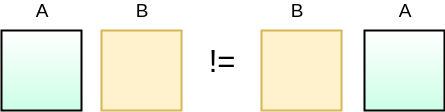
\includegraphics[scale =0.3]{square_mat_commutation.png}\\
	   \end{center}
	\item For a valid matrix multiplication operation, the matrix dimensions must agree: the number of columns in the first matrix should be equal to number of rows in the second matrix. \\
		\begin{center}
	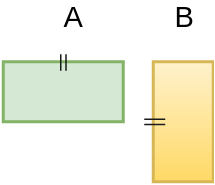
\includegraphics[scale =0.3]{matrix_commutation.png}\\
	    \end{center}
	\item When more than two matrices are multiplied, it is called  matrix chain multiplication. \\ 
		\begin{center}
		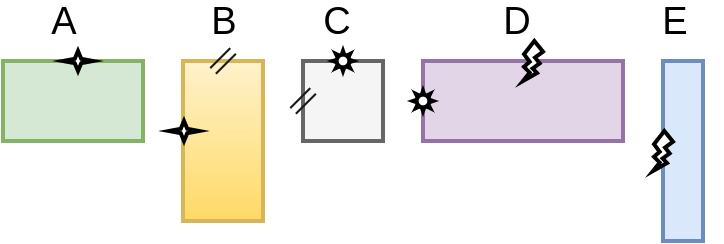
\includegraphics[scale =0.2]{chain_matrix.png}
	\end{center}
\end{enumerate} 

Further we note the following points: In this project we consider a matrix that is filled with double precision real numbers and all the computations were performed using highly optimized library OpenBLAS [1]


\section{Problem formulation}

\subsection*{Toy problem} 
 To begin with, we consider a chain with 3 matrices. We have three random matrices A, B, C of sizes $10*30, 30*5, 5*60$ respectively. If we want to multiply these matrices, there are two possible ways.
 This is illustrated in figure \ref{fig:3mat_1_full} .  
 
 
 \begin{figure}[h!]	
 	\begin{center}
 	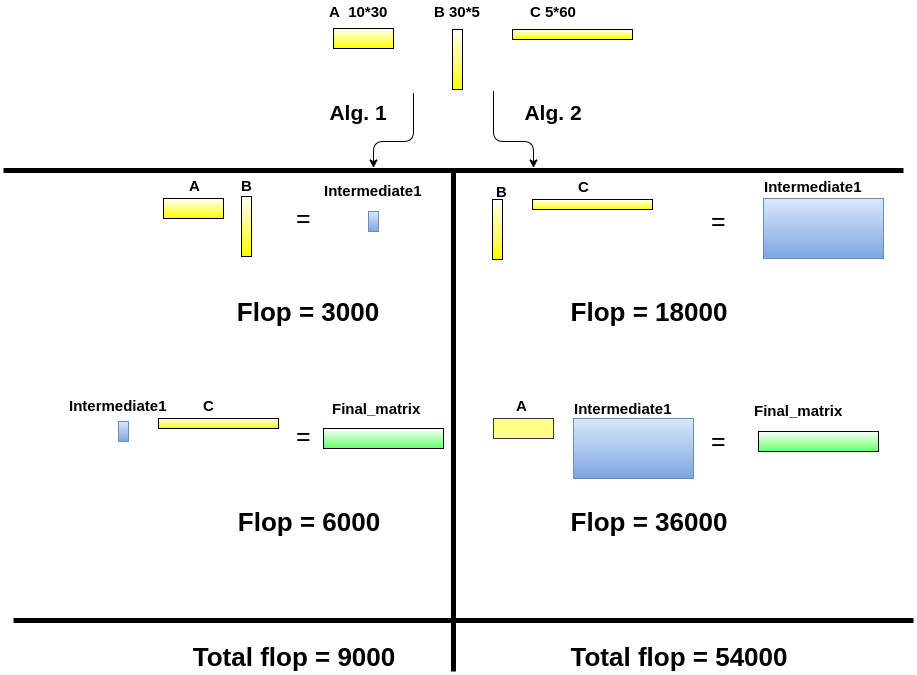
\includegraphics[scale =0.4]{3mat_1_full.png}
 	\caption{Two possible ways of multiplying 3 matrices}
 	\label{fig:3mat_1_full}
    \end{center}
  \end{figure}
In algorithm 1 we multiply the matrices A and B first. Then with the intermediate result we multiply the third matrix C. Whereas in algorithm 2 we start with matrices B and C first and then we multiply the intermediate result with the matrix A. In both ways we obtain the same end result but the main difference lies in amount of flop\footnote{Flop is a quantity which tells how many number of arithmetic operations are performed in computation} performed in order to obtain the end result. From figure \ref{fig:3mat_1_full} we can infer that the algorithm 2 is 6 times costlier than the algorithm 1 but which algorithm executes faster? We defer such delicate question related to execution time to later sections.     



\subsection*{Main problem}
Now we move from a simple toy example to a sophisticated problem. We consider 5 matrices of random sizes A,B,C,D,E.
 \begin{figure}[h!]
 		\begin{center}
    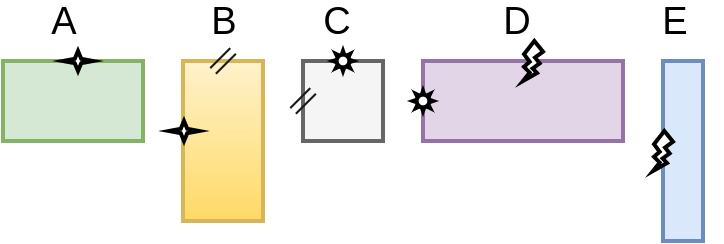
\includegraphics[scale =0.3]{chain_matrix.png}
 	\caption{5 matrices chain}
 	\label{fig:chain_matrix}
 	\end{center}
 \end{figure}


We want to multiply these matrices. To do so, we multiply matrices A,B first. Then with the first intermediate result we multiply C and then with the second intermediate result we multiply matrix D and finally with the third intermediate results we multiply E. This is
possibility-1	(((A*B)*C)*D)*E  but there is also another possibility. We can start with matrices D, E and do the same but in reverse order. This is possibility-2	A*(B*(C*(D*E))). There are many more such possibilities. There exists a set up which allows to find all the possibilities. It is called Catalan number and parenthesization problem [2]. \\
	$P_n$ parenthesization: $P_n = C_{n-1}$ \\ 
	$n^{th}$ Catalan number : $C_n = \frac{1}{n+1} \binom{2n}{n}$ \\

\begin{table}[htp!]
	\centering
\begin{center}
	\begin{tabular}{| c |c |c| c| c| c| c| c| c| c |}
		\hline 
		n  & 2 & 3 & 4 & 	\textcolor{red}{5} & 6 & 7 & 8 & 9\\ [1ex]
		\hline 
		$P_n$ & 1 & 2 & 5 & \textcolor{red}{14} & 42 & 132 & 429 & 1430\\[1ex]
		\hline
	\end{tabular}
\end{center} 
	\caption{Catalan number and paranthesization}
	\label{table:Catalan number and paranthesization}
\end{table}


	
The above set up gives us possibility to count all ways to group n factors with parenthesis. Using that, we formed the following 14 possibilities.
\begin{center}
	\textcolor{red}{Alg.-0} (((A*B)*C)*D)*E \\ 
	\textcolor{red}{Alg.-1} (A*(B*(C*D)))*E\\
	\textcolor{red}{Alg.-2} A*(B*(C*(D*E)))\\
	\textcolor{red}{Alg.-3} A*(((B*C)*D)*E)\\
	\textcolor{red}{Alg.-4} A*((B*C)*(D*E))\\
	\textcolor{red}{Alg.-5} A*(B*((C*D)*E))\\
    \textcolor{red}{Alg.-6} A*((B*(C*D))*E) \\
	\textcolor{red}{Alg.-7} (A*B)*(C*(D*E))\\
	\textcolor{red}{Alg.-8} (A*B)*((C*D)*E) \\
	\textcolor{red}{Alg.-9} ((A*B)*C)*(D*E)\\
	\textcolor{red}{Alg.-10} (A*(B*C))*(D*E)\\
	\textcolor{red}{Alg.-11} ((A*(B*C))*D)*E\\
	\textcolor{red}{Alg.-12} (A*((B*C)*D))*E\\
	\textcolor{red}{Alg.-13} ((A*B)*(C*D))*E\\
\end{center}

For better understanding we visualized all the algorithms as block diagrams. See Figure \ref{fig:5mat_color_black_Arrow}.

\begin{figure}[h!] 
	\begin{center}
	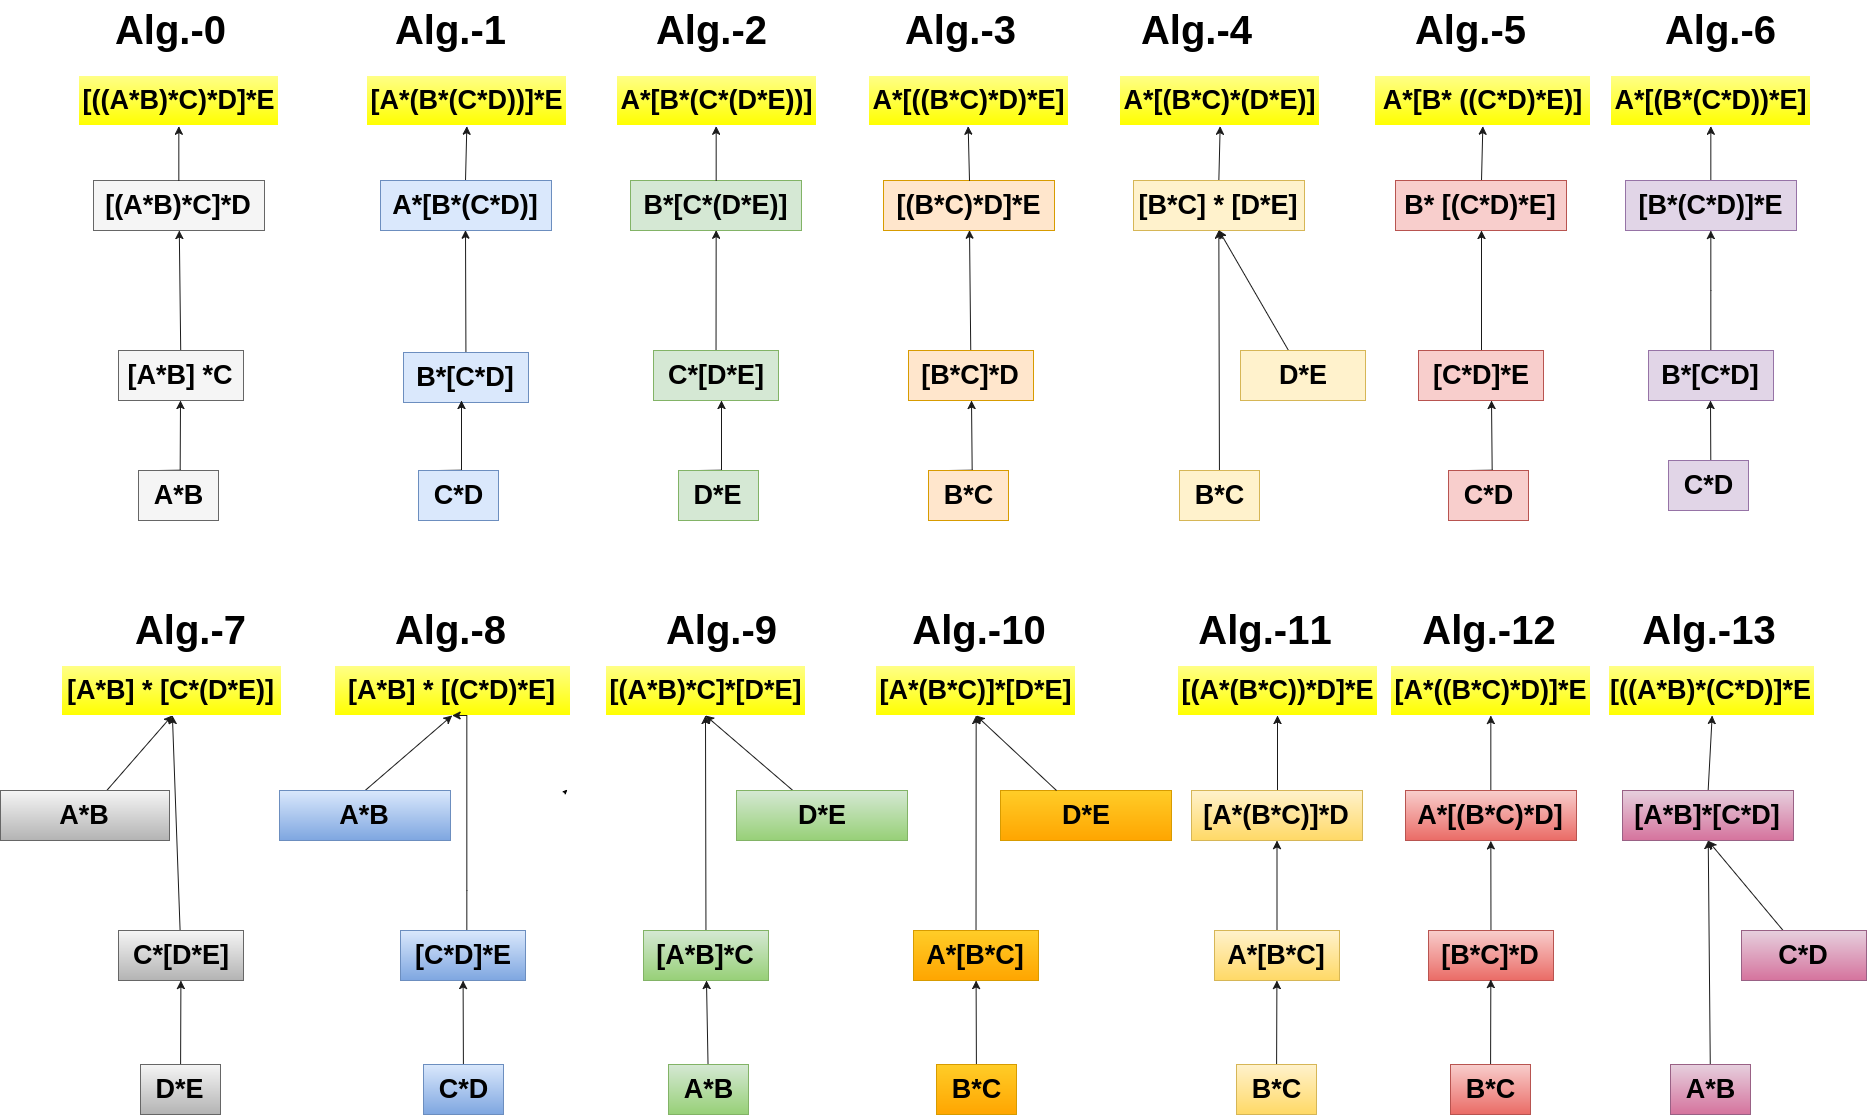
\includegraphics[scale =0.25]{5mat_color_black_Arrow.png}
   	\caption{14 possible algorithms for 5 matrices chain}
   	\label{fig:5mat_color_black_Arrow}
   	\end{center}
\end{figure}
	
The two main questions we want to ask ourselves are as follows: out of all algorithms which algorithm performs minimum number of flop?, which algorithm takes minimum time to execute? We are also interested in a quantity "deviation" which is described below. 


	\begin{enumerate}[(\roman{*})]
		\item \textbf{Flop} - How many floating point operations does each algorithm perform? \\
    	\textcolor{red}{min\textunderscore flop\textunderscore alg}   - Algorithm which performs minimum flop\\
		\item \textbf{Execution time (in Seconds)} - How much time does each algorithm take to execute?\\
		\textcolor{blue}{min\textunderscore time\textunderscore alg}   - Algorithm which takes minimum time to execute\\
		\item $\textbf{Deviation (in \%)}\\
		Deviation =\frac{t_{min \textunderscore flop \textunderscore alg}-t_{min\textunderscore time \textunderscore alg}}{t_{min \textunderscore time \textunderscore alg}} *100$ \\
		How much percentage is the "$min\textunderscore time\textunderscore alg$" faster than the "$min\textunderscore flop\textunderscore alg$" ? \\
     	\textcolor{red}{$t_{min \textunderscore flop \textunderscore alg}$} - time for minimum flop algorithm\\
		\textcolor{blue}{$t_{min\textunderscore time \textunderscore alg}$}  -  time for minimum time algorithm
	\end{enumerate}


\subsection*{Pseudo algorithm}
We have written a software application, in C programming language, which gives us the results of questions that are addressed in the previous section. For more details refer [3].


\begin{center}
 \begin{lstlisting}[language=c++]
 main { 
 Timer start
 Alg. 0}
 Timer finish
 Timer start
 Alg. 1
 Timer finish
 .
 .
 . 				 
 Timer start
 Alg. 13
 Timer finish
      }
 \end{lstlisting}
\end{center}


Input  : 
\hspace{2pt}Matrix sizes$[1,2,3,4,5,6]$\\ 
output :\\
\begin{tabular}{ c c }
	time\textunderscore 0 & flop\textunderscore 0 \\ 
	time\textunderscore 1 & flop\textunderscore 1 \\ 
	time\textunderscore 2 & flop\textunderscore 2 \\ 
	. & .\\
	. & .\\
	time\textunderscore 12 & flop\textunderscore 12 \\
	time\textunderscore 13 & flop\textunderscore 13 
\end{tabular}\\
Min\textunderscore flop\textunderscore alg\\
Min\textunderscore flop\textunderscore alg\\
Deviation\\

\subsection*{Test cases}
\begin{figure}[h!]	
	\begin{center}
		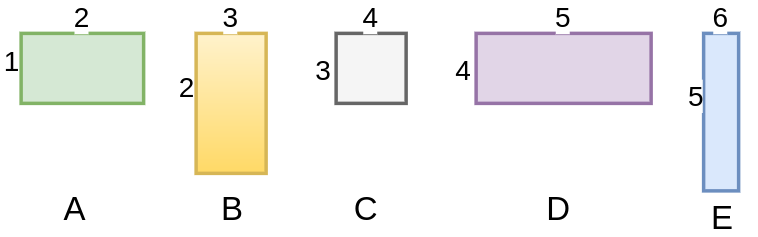
\includegraphics[scale =0.3]{chain_matrix_numero.png}
		\caption{5 matrices chain}
		\label{fig:5 matrices chain with number}
	\end{center}
\end{figure}

As a test case we consider two chains randomly. First chain consists of matrices of different sizes, size ranges size from 100 to 1300 and second one consists of matrices of more or less same sizes.\\ 
$1^{st}$ Chain   130 700 383 1340 193 900\\
$2^{nd}$ Chain   376 561 477 532 425 590 



\section{Results and Discussion}
In this section we look at the results of our problem. We use the following notations, throughout the text, chain\footnote{Chain refers to matrix chain and specifies whether it is $1^{st}$ or $2^{nd} $chain } and run\footnote{It is $n$ repetition of experiment with the same input} for the sake of simplicity. we conducted 50 runs for each chain. We present only 3 run-results for each chain out of 50 runs.     	
	
\subsection*{$1^{st}$ Chain (Run-1)  }

 \begin{table}[htp!]
 	\centering
 	\begin{center}
 		\begin{tabular}{| l | l | l |}
 			\hline
 			\textbf{Algorithm}  & \textbf{Time} (seconds) & \textbf{Flop}\\
 			\hline		
 			0	&   0.051306	&	\textcolor{red}{315,546,400}\\
 			1	&	0.065909 	&	381,877,520\\
 			2 	&	0.247766 	&	2,035,692,000\\
 			3 	&	0.180365 	&	1,487,556,000 \\
 			4 	&	0.361984 	&	3,036,224,000\\
 			5 	&	0.118680 	&	977,537,120\\
 			6	&    0.088250 	&	708,569,520\\
 			7 	&	0.185151 	&	1,548,640,000\\
 			8 	&	0.061688 	&	490,485,120\\
 			9 	&	0.122389 	&	982,219,200\\
 			10 	&	0.215232 	&	1,741,464,000\\
 			11 	&	0.131261 	&	1,074,791,200\\
 			12 	&	0.140059 	&	1,160,864,000\\
 			13 	&	\textcolor{blue}{0.042321} 	&	332,189,860	\\[1ex]
 			\hline
 		\end{tabular}		
 	\end{center}
 	\caption{$1^{st}$ Chain (Run-1)}
 	\label{table:$1^{st}$ Chain (Run-1)}
 \end{table}


 First run result of first chain is presented in table \ref{table:$1^{st}$ Chain (Run-1)}, we see that \textcolor{red}{min\textunderscore flop\textunderscore alg} is $0$,
 \textcolor{blue}{min\textunderscore time\textunderscore alg} is $13$ and  \textcolor{black}{deviation is 21.2\%}. That means the algorithm 13 is 21.2\% faster than the algorithm $0$, even though it performs more flop than algorithm 0.
 


\subsection*{$1^{st}$ Chain (Run-2)  }
We repeated the experiment and obtained the results in table \ref{table:$1^{st}$ Chain (Run-2)}. We see that this time \textcolor{red}{min\textunderscore flop\textunderscore alg} is $0$, \textcolor{blue}{min\textunderscore time\textunderscore alg} is $0$ and  \textcolor{black}{deviation is 0.0\%}. That means the algorithm 0 is the fastest among all. 
 \begin{table}[htp!]
 	\centering
 	\begin{center}
 	\begin{tabular}{| l | l | l |}
 		\hline
 		\textbf{Algorithm}  & \textbf{Time} (seconds) & \textbf{Flop}\\
 		\hline
 		0 	&	\textcolor{blue}{0.042322} 	&	\textcolor{red}{315,546,400} \\			
 		1 	&	0.054053 	&	381,877,520 	\\	
 		2 	&	0.255563 	&	2,035,692,000 	\\	
 		3 	&	0.187326 	&	1,487,556,000 	\\		
 		4 	&	0.381132 	&	3,036,224,000 	\\		
 		5 	&	0.120140 	&	977,537,120 	\\		
 		6 	&	0.087574 	&	708,569,520 	\\		
 		7 	&	0.189211 	&	1,548,640,000 	\\		
 		8 	&	0.061826 	&	490,485,120 	\\		
 		9 	&	0.151340 	&	982,219,200 	\\		
 		10 	&	0.274111 	&	1,741,464,000 	\\		
 		11 	&	0.178278 	&	1,074,791,200 	\\		
 		12 	&	0.181404 	&	1,160,864,000 	\\		
 		13 	&	0.045157 	&	332,189,860	\\
 		\hline
 	\end{tabular}		
 	\end{center}
 	\caption{$1^{st}$ Chain (Run-2)}
 	\label{table:$1^{st}$ Chain (Run-2)}
 \end{table}
\subsection*{$1^{st}$ Chain (Run-3)  } 
 We consider one more sample result before moving on to next chain. From table \ref{table:$1^{st}$ Chain (Run-3)}, we see that this time again the \textcolor{red}{min\textunderscore flop\textunderscore alg} is $0$, \textcolor{blue}{min\textunderscore time\textunderscore alg} is $13$ and  \textcolor{black}{deviation is 25.4\%}. That means the algorithm 13 is 25.4\% faster than the algorithm $0$, even though it performs more flop than algorithm 0.
\begin{table}
 	\centering
 	\begin{center}
 			\begin{tabular}{| l | l | l |}
 				\hline
 				\textbf{Algorithm}  & \textbf{Time} (seconds) & \textbf{Flop}\\
 				\hline	
 				0 	&	0.055871 	&	\textcolor{red}{315,546,400} 	\\		
 				1 	&	0.056499 	&	381,877,520 	\\		
 				2 	&	0.261406 	&	2,035,692,000 	\\		
 				3 	&	0.206040 	&	1,487,556,000	\\		
 				4 	&	0.387012 	&	3,036,224,000	\\		
 				5 	&	0.131321 	&	977,537,120 	\\		
 				6 	&	0.092505 	&	708,569,520 	\\		
 				7 	&	0.196337 	&	1,548,640,000 	\\		
 				8 	&	0.066044 	&	490,485,120 	\\		
 				9 	&	0.128545 	&	982,219,200	\\		
 				10 	&	0.226485 	&	1,741,464,000 	\\		
 				11 	&	0.137919 	&	1,074,791,200	\\		
 				12 	&	0.146254 	&	1,160,864,000 	\\		
 				13 	&	\textcolor{blue}{0.044547} 	&	332,189,860 \\
 				\hline
 			\end{tabular}		
 	\end{center}
 	\caption{$1^{st}$ Chain (Run-3)}
 	\label{table:$1^{st}$ Chain (Run-3)}
 \end{table}

\subsection*{$2^{nd}$ Chain (Run-1) } 
First run results of second chain is presented in table \ref{table:$2^{nd}$ Chain (Run-1)}. We observe similar phenomenon for the $2^{nd}$ chain too. For each run we observed different results. We see the result of first run of second chain. The \textcolor{red}{min\textunderscore flop\textunderscore alg} is $0$, \textcolor{blue}{min\textunderscore time\textunderscore alg} is $13$ and  \textcolor{black}{deviation is 8.44\%}. 
 
    
    \begin{table}[htp!]
    	\centering
    	\begin{center}
    	\begin{tabular}{| l | l | l |}
    		\hline
    		\textbf{Algorithm}  & \textbf{Time} (seconds) & \textbf{Flop}\\
    		\hline	
    			0 & 0.101891 &\textcolor{red}{750,654,672}\\ 		
    			1 &	0.099232 &	811,016,450 \\	
    			2 &	0.140206 &	1,130,908,460 \\		
    			3 &	0.130707 &	1,068,653,388\\
    			4 &	0.139825 &	1,152,599,048 \\		
    			5 &	0.126232 &	1,019,583,840	\\	
    			6 &	0.121548 &	973,402,830 	\\	
    			7 &	0.121522 &	979,107,824	\\	
    			8 &	0.110458 &	867,783,204	\\	
    			9 &	0.112590 &	894,899,232 	\\	
    			10 &	0.124695 &	1,011,994,872 \\		
    			11 &	0.106382 &	867,750,312 	\\	
    			12 &	0.112451 &	906,267,008 	\\	
    			13 &    \textcolor{blue}{0.093955} &757,945,544	\\
    			\hline
    		\end{tabular}		
    	\end{center}
    	\caption{$2^{nd}$ Chain (Run-1)}
    	\label{table:$2^{nd}$ Chain (Run-1)}
    \end{table}
    
\newpage   
	
\subsection*{$2^{nd}$ Chain (Run-2)  }
For the second run, from table \ref{table:$2^{nd}$ Chain (Run-2)}, we observe that this time \textcolor{red}{min\textunderscore flop\textunderscore alg} is $0$, \textcolor{blue}{min\textunderscore time\textunderscore alg} is $0$ and  \textcolor{black}{deviation is 0.0\%}. That means the algorithm 0 is the fastest among all.  
\begin{table}[htp!]
	\centering
	\begin{center}
		
	\begin{tabular}{| l | l | l |}
		\hline
		\textbf{Algorithm}  & \textbf{Time} (seconds) & \textbf{Flop}\\
		\hline			
			0 &	\textcolor{blue}{0.090527} &	\textcolor{red}{750,654,672}\\ 		
			1 &	0.096886 &	811,016,450 \\		
			2 &	0.133695 &	1,130,908,460 	\\	
			3 &	0.126657 &	1,068,653,388 	\\
			4 &	0.137426 &	1,152,599,048 	\\	
			5 &	0.122484 &	1,019,583,840 	\\	
			6 &	0.116337 &	973,402,830 	\\	
			7 &	0.122186 &	979,107,824 	\\	
			8 &	0.113717 &	867,783,204 	\\	
			9 &	0.109312 &	894,899,232 	\\	
			10 &	0.123241& 	1,011,994,872\\ 		
			11 & 0.105787 	&867,750,312 		\\
			12 &	0.110508 &	906,267,008 	\\	
			13 &	0.091250 &	757,945,544  	\\	
			\hline
		\end{tabular}
	\end{center}
	\caption{$2^{nd}$ Chain (Run-2)}
	\label{table:$2^{nd}$ Chain (Run-2)}
\end{table}


\subsection*{$2^{nd}$ Chain (Run-3)  } 
For the third run,from table \ref{table:$2^{nd}$ Chain (Run-3)}, we see that, again the \textcolor{red}{min\textunderscore flop\textunderscore alg} is $0$, \textcolor{blue}{min\textunderscore time\textunderscore alg} is $13$ and  \textcolor{black}{deviation is 9.12\%}.

\begin{table}[htp!]
	\centering
	\begin{center}
	\begin{tabular}{| l | l | l |}
		\hline
		\textbf{Algorithm}  & \textbf{Time} (seconds) & \textbf{Flop}\\
		\hline		
			0 &	0.102252 &	\textcolor{red}{750,654,672} 	\\	
			1 &	0.114649 &	811,016,450 	\\	
			2 &	0.145311 &	1,130,908,460 	\\	
			3 &	0.129112 &	1,068,653,388 	\\	
			4 &	0.139820 &	1,152,599,048 	\\	
			5 &	0.129094 &	1,019,583,840 	\\	
			6 &	0.120107 &	973,402,830 	\\	
			7 &	0.120611 &	979,107,824 	\\	
			8 &	0.107226 &	867,783,204 	\\	
			9 &	0.110580 &	894,899,232 	\\	
			10 &	0.123456& 	1,011,994,872 \\ 		
			11 	&0.105604 	&867,750,312 		 \\
			12 	&0.110942 	&906,267,008 		\\
			13 	& \textcolor{blue}{0.093701} 	&757,945,544	\\
			\hline
		\end{tabular}\\
	\end{center}
	\caption{$2^{nd}$ Chain (Run-3)}
	\label{table:$2^{nd}$ Chain (Run-3)}
\end{table} 




Considering all the run results that we have seen so far, we need no explanation when the $min\textunderscore flop\textunderscore alg$ is the fastest but we want to understand what happens in the other cases. i.e, the cases when there is an algorithm with more flop executes faster. This happens because all flop do not cost the same.  This leads us to the next section which verifies this statement.
	
\subsection*{All flops do not cost the same}
 Let us consider multiplication of two square matrices. We recorded Flops for different matrix sizes from 100 to 3000. 


\begin{table}[htp!]
	\centering
			\begin{center}
				\begin{tabular}{| l| l |l | }
					\hline
					\textbf{Size of A,B} & \textbf{Flop} & \textbf{FLOPS = $\frac{Flop}{Second}$}  \\ 
					\hline
					$(100*100)$ &  2,000,000    &  4,672,897,196\\ 
					$(200*200)$ &  16,000,000   &  4,705,882,352\\ 
					$(300*300)$ &  54,000,000   &  5,819,592,628\\
					$(400*400)$ &  128,000,000  & 6,994,535,519\\
					..  &  ... & ...\\
					..  &  ...&...\\
					..  &  ...&...\\
					$(1300*1300)$&  4,394,000,000&7,036,896,462\\
					$(1400*1400)$&  5,488,000,000&7,109,296,363 \\
					$(1500*1500)$&  6,750,000,000&7,048,975,235\\
					...& ...& ...\\
					$(3000*3000)$&  54,000,000,000&7,404,131,916\\
					\hline
				\end{tabular} 
			\end{center}
	\caption{Matrix size vs FLOPS}
	\label{table:Matrix size vs FLOPS}
\end{table} 

 We plotted a graph for number of flops against matrix sizes. Refer figure \ref{fig:benchmarkcurve}.  What we can observe from figure \ref{fig:benchmarkcurve} is that when we give large matrices, more flops are performed in opposition to small matrix sizes. To emphasize, when we multiply two matrices of size $100*100$
 the machine performs approximately $4.6*10^{9}$ Flop per second but when we multiply, for instance $3000*3000$ matrices the machine does not restrict itself to the value $4.6*10^{9}$ rather it performs $7.4*10^{9}$ Flop per second. We conclude this section by verifying that, indeed all flops do not cost the same.\\
  \begin{figure}[!]
 		\begin{center}
 	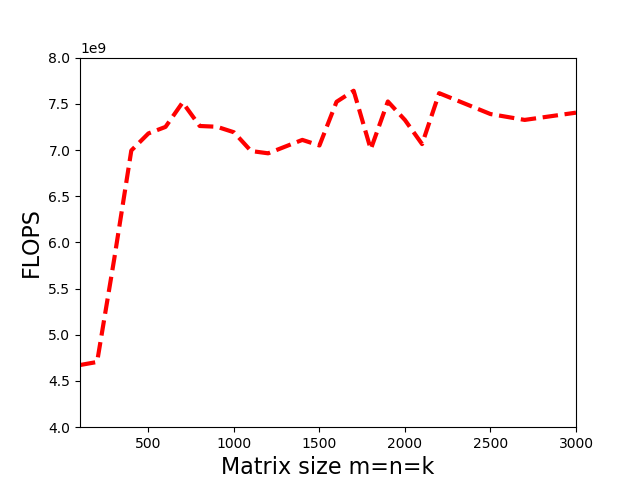
\includegraphics[scale =0.9]{benchmarkcurve.png}
 	\caption{All flops do not cost the same}
 	\label{fig:benchmarkcurve}
 	\end{center}
 \end{figure}


\section{Perturbation analysis}
\subsection*{Goal}
From previous sections we saw that some of the quantities that we are interested in such as execution time and deviation  are not reproducible. So we conducted several runs for the same input. i.e., we gave $1^{st}$ chain as input and repeated the experiment 50 times for same input and recorded following quantities:
		\begin{enumerate}[(\roman{*})] 
				\item \textbf{Deviation frequency}: It shows us, out of 50 iterations how often does deviation occur? In others words, how often the  $min\textunderscore flop\textunderscore alg$ and  $min\textunderscore time\textunderscore alg$ are not the same?
	            \item \textbf{Deviation range}: It reflects, out of 50 iterations, if deviation occurs, then what is the minimum deviation and the maximum deviation? 
	
				\item \textbf{Flop difference}: It shows the flop difference between the  $min\textunderscore flop\textunderscore alg$ and  the $min\textunderscore time\textunderscore alg$. 
	   \end{enumerate}
	   Now we want to perturb the  matrix chain i.e., we consider a new chain in the neighborhood of unperturbed matrix chain. If we look carefully, we see that each matrix chain has 6 elements in it. We want to perturb each element by same amount and find a new chain. For example, if our unperturbed chain was 130 700 383 1340 193 900 and we perturbed each element by 1\% , then we would get a new chain as 131 707 386 1353 198 909. We consider range from -15\% to +15\%. For each new chain we conducted equal number of runs as we did for our original chain and we want to study what happens to the quantities that we defined earlier in the section.


\subsection*{$1^{st}$ Chain \hspace{10pt} \textit{All elements perturbation}}
     	\begin{table}[h!]
     		\centering
     		
     			\begin{tabular}{|c| c | c |c | c |}
     				\hline
     				\textbf{Perturbation} &\textbf{Matrix} & \textbf{Deviation} & \textbf{Deviation} & \textbf{Flop }\\
     				\textbf{percentage}&\textbf{chain}& \textbf{range}&\textbf{frequency}&\textbf{difference}\\
     				\hline
     					\textcolor{green}{+15\%}&149 805 440 1541 221 1035	&	 0.01-29 \%		&	25\%		&	25,128,102\\
     				\textcolor{green}{+10\%}&143 770 421 1474 152 990	&	 3.5-15 \%		&	8\%			&   21,006,788\\
     				\textcolor{green}{+5\%}&136 735 402 1407 202 945	&    0.01-68 \%		&	30\%		&	19,442,328\\
     			\textcolor{green}{+3\%}	&133 721 394 1380 198 927	&    0.01-40 \%		&	40\%		&	18,752,952\\
     			\textcolor{green}{+1\%}	&131 707 386 1353 194 909	&    0.01-18.5\%	&	40\%	    &	16,653,820\\
     			\textcolor{blue}{Unperturbed}	&\textcolor{blue}{130} \textcolor{blue}{700} \textcolor{blue}{383} \textcolor{blue}{1340} \textcolor{blue}{193} \textcolor{blue}{900}	&    \textcolor{blue}{0.01-36 \%}		&	\textcolor{blue}{27\%}		&	\textcolor{blue}{16,643,460}\\
     			\textcolor{red}{-1\%}	&128 693 379 1326 191 891	&    0.01-21 \%		&	26\%		&	17,017,292\\
     			\textcolor{red}{-3\%}	&126 679 371 1299 187 873	&    0.01-42 \%		&	30\%		&	15,064,266\\
     			\textcolor{red}{-5\%}	&123 665 363 1273 183 855	&    0.01-80 \%		&	34\%		&	14,485,500\\
     			\textcolor{red}{-10\%}	&117 630 344 1206 173 810	& 	 0.01-22 \%		&	30\%		&	11,569,284\\
     			\textcolor{red}{-15\%}	&110 595 325 1139 164 765	&	 0.01-18 \%		&	28\%		&	10,609,780\\
     				\hline	
     			\end{tabular}
     	
     		\caption{$1^{st}$ Chain - All elements perturbation}
     		\label{table:$1^{st}$ Chain - All elements perturbation}
     	\end{table}
   
    \vspace*{4pt} 
     	The table \ref{table:$1^{st}$ Chain - All elements perturbation} shows results of perturbation of $1^{st}$ chain. The blue colored row represents unperturbed chain. The rows which are placed above and below the unperturbed chain, are  perturbed in an increasing and decreasing manner respectively. For the unperturbed chain deviation frequency is around 27\% out of 50 runs and the deviation range is from 0.01 \% to 36\%. We see that, for all perturbed chains there is corresponding  deviation frequency and the maximum value is limited to 40\%. Particularly, in the case of +10\% perturbation deviation occurrence is rare and it is only about  8\% out of 50 runs.
     	
     	After a closer examination of the deviation range, we find a pattern in behavior of deviation range with respect to perturbation percentage. For small perturbation percentage, this parameter drops and then it increases rapidly. Once it reaches maximum value, it drops again. It is the case for both, positive and negative perturbations.
     	
     	One interesting point to consider is, perturbation with 5\% in both positive and negative directions gives us the highest deviation range which is about 68\% and 80\% respectively and approximately 2 times greater than the original chain's value.



\subsection*{$2^{nd}$ Chain \hspace{10pt} \textit{All elements perturbation}}
        We carried out a similar study for the second chain. The results of perturbation of $2^{nd}$ chain is shown in table \ref{table:$2^{nd}$ Chain - All elements perturbation}. The values are placed like in the previous case.
        
         \begin{table}[htp!]
         	\centering
         	
         	
         	\begin{tabular}{|c| c | c |c | c |}
         		\hline
         		\textbf{Perturbation} &\textbf{Matrix} & \textbf{Deviation} & \textbf{Deviation} & \textbf{Flop }\\
         		\textbf{percentage}&\textbf{chain}& \textbf{range}&\textbf{frequency}&\textbf{difference}\\
         		\hline
         		\textcolor{green}{+15\%}	&432 645 548 611 488 678	&	0.01-15 \%		&	46.5\%	&		10,937,920\\
         		\textcolor{green}{+10\%}	&413 617 524 585 467 649	&	3.5-6\%			&    48\%	&		9,576,058\\
         		\textcolor{green}{+5\%}	&394 589 500 558 446 619 &	0.01-67 \%		&	52.5\%	&		8,632,016\\
         		\textcolor{green}{+3\%}	&387 577 491 547 437 607	&	0.01-20 \%		&	43\%	&		7,916,372\\
         		\textcolor{green}{+1\%}	&379 566 481 537 429 595 &	0.01-19 \%		&	63\%	&		7,619,508\\
         		\textcolor{blue}{Unperturbed}	&\textcolor{blue}{376} \textcolor{blue}{561} \textcolor{blue}{477} \textcolor{blue}{532} \textcolor{blue}{425} \textcolor{blue}{590}	&    \textcolor{blue}{0.01-22 \%}		&	\textcolor{blue}{40\%}		&	\textcolor{blue}{7,290,872}\\
         		\textcolor{red}{-1\%}	&372 555 472 526 420 584	&	0.01-13 \%		&	65\%	&		6,960,192\\	
         		\textcolor{red}{-3\%}	&364 544 462 516 412 572 &	0.01-20 \%		&	47.5\%	 &		6,89,088\\
         		\textcolor{red}{-5\%}	&357 532 453 505 403 560	&	0.01-73 \%		&	57\%	 &		6,083,796\\
         		\textcolor{red}{-10\%}	&338 504 429 478 382 531	&	0.01-34 \%		&	43\%   	 &		5,392,088\\
         		\textcolor{red}{-15\%}	&319 476 405 452 361 501	&	0.01-19 \%		&	40\%	 &		4,552,094\\
         		\hline
         	\end{tabular}
         	
         	
         	\caption{$2^{nd}$ Chain - All elements perturbation}
         	\label{table:$2^{nd}$ Chain - All elements perturbation}
         \end{table}
         	
    \vspace*{4pt}     	
         	 Interestingly, we observe similar patterns for this chain as well. We see that flop difference increases with increasing matrix sizes. The difference in deviation frequency among all chains, is not very much, values ranging from 40\% up to 65\%. In the case of deviation range, we see the similar behavior like for the $1^{st}$ chain,  For small perturbation percentage, this parameter drops and then it increases rapidly. Once it reaches the maximum, it drops again. It is the case for both, positive and negative perturbations.

  We saw that significant changes occurred in deviation range and deviation frequency when the chains are perturbed by -5\% and +5\%. It stimulated our curiosity to explore it further. We want to understand what happens when perturbing the chain 5\% and which element of chain contributes to the changes. In other words, we want to find out which elements in a chain are sensitive to perturbation.

\subsection*{$1^{st}$ Chain \hspace{8pt} \textit{Single element perturbation}}
      
      
     Unlike previous perturbations, we perturbed the original chain one element at a time by +5\%. We did the same for negative case also. Results of single element perturbation of $1^{st}$chain is shown in table \ref{table:$1^{st}$ Chain - Single element perturbation}.
        \begin{table}[t!]
        	\centering  	
        	\begin{tabular}{|c| c | c |c | c|}
        		\hline
        		Perturbation&\textbf{Matrix} & \textbf{Deviation} & \textbf{Deviation}& \textbf{Flop }\\
        		percentage&\textbf{chain}  & \textbf{range}     &\textbf{frequency}&\textbf{difference}\\
        		\hline
        		% 130 700 383 1349 193 900 &	0.01-36 \%	&	   27\% 	&		16,643,460\\
        		\textcolor{green}{+5\%}&\textcolor{green}{136} 700 383 1340 193 900 &	0.01-25 \%	&		53\%	&		8,628,408\\
        		\textcolor{green}{+5\%}&130 \textcolor{green}{735} 383 1340 193 900 &	0.01-67 \%	&		33\%	&		16,643,460\\	
        		\textcolor{green}{+5\%}&130 700 \textcolor{green}{402} 1340 193 900 &	0.01-24 \%	&		30\%	&		20,804,840\\	
        		\textcolor{green}{+5\%}&130 700 383 \textcolor{green}{1407} 193 900 &	0.01-74 \%	&		46\%	&		16,514,686\\
        		\textcolor{green}{+5\%}&130 700 383 1340 \textcolor{green}{202} 900 &	2 - 21 \%		&     	26\%	&		23,642,040\\
        		\textcolor{green}{+5\%}&130 700 383 1340 193 \textcolor{green}{945} &	1 - 40 \%		&	    36\%	&		16,643,460\\
        		\textcolor{blue}{Unperturbed}& \textcolor{blue}{130} \textcolor{blue}{700} \textcolor{blue}{383} \textcolor{blue}{1340} \textcolor{blue}{193} \textcolor{blue}{900} &	\textcolor{blue}{0.01-36 \%}	  &	    \textcolor{blue}{27\%}	&		\textcolor{blue}{16,643,460}\\
        		\textcolor{red}{-5\%}& \textcolor{red}{123} 700 383 1340 193 900 &	0.01-50 \%	  &		23\%	&		26,414,454\\
        		\textcolor{red}{-5\%}&130 \textcolor{red}{665} 383 1340 193 900 &	0.01-85 \%	  &		56\%	&		16,643,460\\	
        		\textcolor{red}{-5\%}&130 700 \textcolor{red}{363} 1340 193 900 &	0.01-13 \%	  & 	43\%	&		9,263,060\\
        		\textcolor{red}{-5\%}&130 700 383 \textcolor{red}{1273} 193 900 &	4 - 84 \%		  &	    30\%	&		16,772,234\\
        		\textcolor{red}{-5\%}&130 700 383 1340 \textcolor{red}{183} 900 &	0.01-26\%	  &		56\%	&		 8,867,260\\
        		\textcolor{red}{-5\%}&130 700 383 1340 193 \textcolor{red}{855} &	0.01-39 \%	  &	    36\%	&		16,643,460\\
        		\hline
        	\end{tabular}  	
        	\caption{$1^{st}$ Chain - Single element perturbation}
        	\label{table:$1^{st}$ Chain - Single element perturbation}
        \end{table}

\vspace*{4pt}

Blue colored row represents the unperturbed chain. The first column indicates how much percentage each element is perturbed. In our case it is 5\%. The rows which are above original chain are incremented by 5\% whereas rows below the original chain are decremented by 5\%. It is shown by corresponding symbol + or -. The second column shows which element of the chain is perturbed and rest of quantities are same as we discussed earlier. Overall we can see that this chain is sensitive to single element perturbation.

For unperturbed chain the deviation range is 0.01\%-36\% and deviation frequency is 27\%.  When we perturb the $2^{nd}$ and $4^{th}$ elements by +5\% the deviation range is increased twice in comparison with original deviation range and deviation frequency is considerably higher. Similarly when we perturb the $2^{nd}$ and $4^{th}$ elements by -5\% the deviation range is increased almost thrice compared to original deviation range and deviation frequency is considerably higher. On the other hand when we perturb the $3^{rd}$ element by +5\% and -5\% the deviation range is lower than the original values.

If we look at flop difference of unperturbed chain, it is 16,643,460. When we perturb $1^{st}$ element by -5\% , flop difference is increased by considerable amount. In fact, it is the highest flop difference among all chain's flop differences. On the contrary when we perturb  $1^{st}$ element by +5\% flop difference reaches the lowest value among all other chain's values.



 \subsection*{$2^{nd}$ Chain \hspace{5pt} \textit{Single element perturbation}}
 We carried out similar study for our second chain also. The results are presented in table \ref{table:$2^{nd}$ Chain - Single element perturbation}.
 \begin{table}[htp!]
 	\centering
 	\begin{tabular}{| c|c | c |c | c |}
 		\hline
 		Perturbation&\textbf{Matrix} & \textbf{Deviation} & \textbf{Deviation} & \textbf{Flop }\\
 		percentage&\textbf{chain}& \textbf{range}&\textbf{frequency}&\textbf{difference}\\
 		\hline
 		\textcolor{green}{+5\%}&\textcolor{green}{394} 561 477 532 425 590	&	0.01-11 \%	 &		23\%	&		2,686,132\\
 		\textcolor{green}{+5\%}&376 	\textcolor{green}{589} 477 532 425 590	&	0.01-17 \%	 &		40\%	&		7,290,872\\	
 		\textcolor{green}{+5\%}&376 561 	\textcolor{green}{500} 532 425 590	&	0.01-49 \%	 &		50\%	&		15,840,800\\	
 		\textcolor{green}{+5\%} &376 561 477 	\textcolor{green}{558} 425 590	&	0.01- 5 \%	 &		23\%	&		   196,668\\
 		\textcolor{green}{+5\%} &376 561 477 532 	\textcolor{green}{446} 590	&	0.01-12\%	 &		30\%	&		17,080,400\\
 		\textcolor{green}{+5\%}&376 561 477 532 425 	\textcolor{green}{619}	&	0.01-16 \%	&		43\%	&		7,290,872\\
 			\textcolor{blue}{Unperturbed}&\textcolor{blue}{376} \textcolor{blue}{561} \textcolor{blue}{477} \textcolor{blue}{532} \textcolor{blue}{425} \textcolor{blue}{590}	&	\textcolor{blue}{0.01-22 \%}	&		\textcolor{blue}{40\%}	&		\textcolor{blue}{7,290,872}\\
 		\textcolor{red}{-5\%} &\textcolor{red}{357} 561 477 532 425 590	  &  	0.01-24 \%		&	26\%		&	17,822,154\\
 		\textcolor{red}{-5\%} &376 	\textcolor{red}{532} 477 532 425 590	  &	    0.01-32 \%		&	41\%		&	7,290,872	\\
 		\textcolor{red}{-5\%} &376 561 	\textcolor{red}{453} 532 425 590	  &	    0.01-11 \%		&	26\%		&	1,630,792	\\
 		\textcolor{red}{-5\%} &376 561 477 	\textcolor{red}{505} 425 590	  &	    0.01-44 \%		&	43\%		&	14,657,930\\
 		\textcolor{red}{-5\%} &376 561 477 532 	\textcolor{red}{403} 590	  &	    0.01- 9 \%		&	26\%		&	2,964,824\\
 		\textcolor{red}{-5\%} &376 561 477 532 425 	\textcolor{red}{560}	  &	    0.01-31 \%		&	43\%		&	7,290,872\\
 		\hline
 	\end{tabular}	
 	\caption{$2^{nd}$ Chain - Single element perturbation}
 	\label{table:$2^{nd}$ Chain - Single element perturbation}
 \end{table} 
         
Surprisingly, we can see somewhat similar phenomenon for this chain as well but main difference lies in the position of element that is sensitive to perturbation. Flop difference of unperturbed chain is 7,290,872. When we perturb $1^{st}$ element by -5\% , flop difference is increased by more than twice. In fact, it is the highest flop difference among all chain's flop differences. On the contrary when we perturb  $4^{st}$ element by +5\% flop difference reaches the lowest value among all other chain's values.

Deviation range of unperturbed chain is 0.01\%-22\% and deviation frequency is 40\%.  When we perturb the $3^{rd}$ elements by +5\% the deviation range is increased twice than the original deviation range and deviation frequency is considerably higher. On the other hand when we perturb the $4^{th}$ and $5^{th}$ element by +5\% and -5\% the deviation range is  much lower than the original value.
 
\section{Conclusion}
Firstly, we studied the relation between flop count and execution time using matrix chain problem as an example problem. Secondly, we also verified that all flops do not cost the same. So when constructing a new algorithm, we should not try to minimize flop of the algorithm for the sake of minimizing execution time. Instead while constructing an algorithm, we should keep the todays computer architecture in our mind and design algorithm accordingly. Finally, we studied the sensitivity of the problem to the perturbation. We also studied crucial elements of the matrix chains.  
\section{Future work}
We conclude this report by giving some pointers to further improvement of this work. In our project we wrote a software application for the problem and tested it using only one node but with the rapid improvement in parallel programming paradigm, we could do even better. We should try to utilize the system capacity as much as possible. There are lot of scope for parallelization in this project. One could parallelize wherever possible and check for timings, flops and deviation.        

%Citations:
\begin{thebibliography}{99}

\bibitem{Item1}
OpenBLAS: An optimized BLAS library. GitHub:  \url{http://www.openblas.net/}

\bibitem{Item2}
Link to Catalan number and parenthesization : \url{https://github.com/edilbert24/Sisc-Lab}

\bibitem{Item3}
Link to the source code : \url{https://github.com/edilbert24/Sisc-Lab}

\bibitem{Item4}
Elmar Peise. {\sl Performance Modeling and Prediction for Dense Linear Algebra}\\ \url{https://arxiv.org/pdf/1706.01341.pdf}

\end{thebibliography}
	

\end{document}


